\documentclass[runningheads,a4paper]{llncs}
\usepackage{amssymb}
\usepackage{amsmath}
\usepackage{placeins}
\setcounter{tocdepth}{3}
\setlength\parindent{24pt}
\usepackage{graphicx}
\usepackage{textcomp}
\usepackage{epstopdf}
\usepackage{listings}
\usepackage{tabularx}
\usepackage{caption}
\usepackage{esvect}
\usepackage{array}
\usepackage[skip=0pt]{caption}
\usepackage[margin=1 in]{geometry}
%\allowdisplaybreaks[1]
%\linespread{1.6}

\newenvironment{sciabstract}{%
\begin{quote} \bf}
{\end{quote}}

\usepackage{url}
\urldef{\mailsa}\path|fry2@case.edu|
\newcommand{\keywords}[1]{\par\addvspace\baselineskip
	\noindent\keywordname\enspace\ignorespaces#1}

\begin{document}

	\mainmatter  % start of an individual contribution
	% first the title is needed
	\title{Thesis Proposal}
	% a short form should be given in case it is too long for the running head
	\titlerunning{Fletcher Young - Thesis Proposal}
	\author{Fletcher Young}%
	%
	\authorrunning{Fletcher Young}
	% (feature abused for this document to repeat the title also on left hand pages)
	% the affiliations are given next; don't give your e-mail address
	% unless you accept that it will be published
	\institute{Case Western Reserve University\\
		Cleveland, OH 44106\\
		\mailsa\\}
	
	\maketitle
	\begin{sciabstract}
		This document is meant to serve as a documentation of research completed thus far.
	\end{sciabstract}

\section{Introduction and Significance}
\section{Background}
\section{Research Strategy}
\subsection{Aim 1 - Develop a physiologically relevant hindlimb model of the rat musculature}
To accomplish this aim, a three dimensional model was created in Animatlab with attachment points and muscle parameters based on data in the literature. The development of this model includes both the biomechanical setup in Animatlab and the code basis to analyze its motion. This model lacks the neural control aspect critical to the project but serves as a platform for biomechanical analysis and development. The development of this model is developed from fundamental principles with each component expanding on the previous development. \par
This model serves as a development of the work completed by Dr. Alex Hunt in completion of his PhD thesis\cite{hunt_development_2017}\cite{hunt_neuromechanical_2014}\cite{hunt_using_2015}. In Dr. Hunt's model, a rat model demonstrated locomotory capabilities through neural control of hindlimb muscles. This work developed the process for decomposing biomechanical movements into the motorneuron signals necessary to generate them. However, this work had the benefit of not having to consider the impact of biarticular muscles, a complication which negates the use of a simple one-to-one CPG to musculature system. In the development of a more biologically relevant model, the inclusion of the full hindlimb musculature must be considered. \par
As a first step in developing a full-muscle hindlimb model, the attachment point of every hindlimb muscle was considered. Initially, this work implemented the attachment points derived by Dr. Will Johnson\cite{johnson_three-dimensional_2008} in which he uses 3D mapping to develop xyz-coordinates for muscle attachment points. The implementation of Johnson’s attachment points were presented as part of a project presentation at Living Machines 2018\cite{young_neuromechanical_2018}. Johnson’s work was useful from an engineering design standpoint but was unusable for two reasons: the coordinates required hand-tuned scaling in order to map correctly onto the existing bone structures and including only the insertion and origins did not accommodate muscle wrapping via points. For this reason, a more nuanced approach was implemented for the muscle attachment points. \par
Muscle paths were defined based on the descriptions by Greene’s 1955 publication Anatomy of the Rat\cite{greene_anatomy_1955}, a primer containing diagrams and descriptions of every system in the rat. Based on this information and the identification of bony landmarks in the 3D bone scans, muscle paths were implemented. Animatlab’s muscle objects are not collision-based, meaning they can pass directly through bones. For muscles that pass closely over bones (such as knee extensors like the vastii muscles), muscle paths include via points. These via points are stationary relative to the bone coordinate frames. \par
Once muscle paths were defined for every muscle, muscle parameters were developed. Animatlab uses a linear Hill muscle, shown in Figure \ref{fig:hill}, model which abides by the equation:
	\begin{align*}
			\frac{dT}{dt} &= \frac{k_{SE}}{c}\bigg[k_{PE}(L-L_{rest})+c \dot{L}-\big(1+\frac{k_{PE}}{k_{SE}}\big)T\bigg]
	\end{align*}
	\begin{figure}
		\centering
		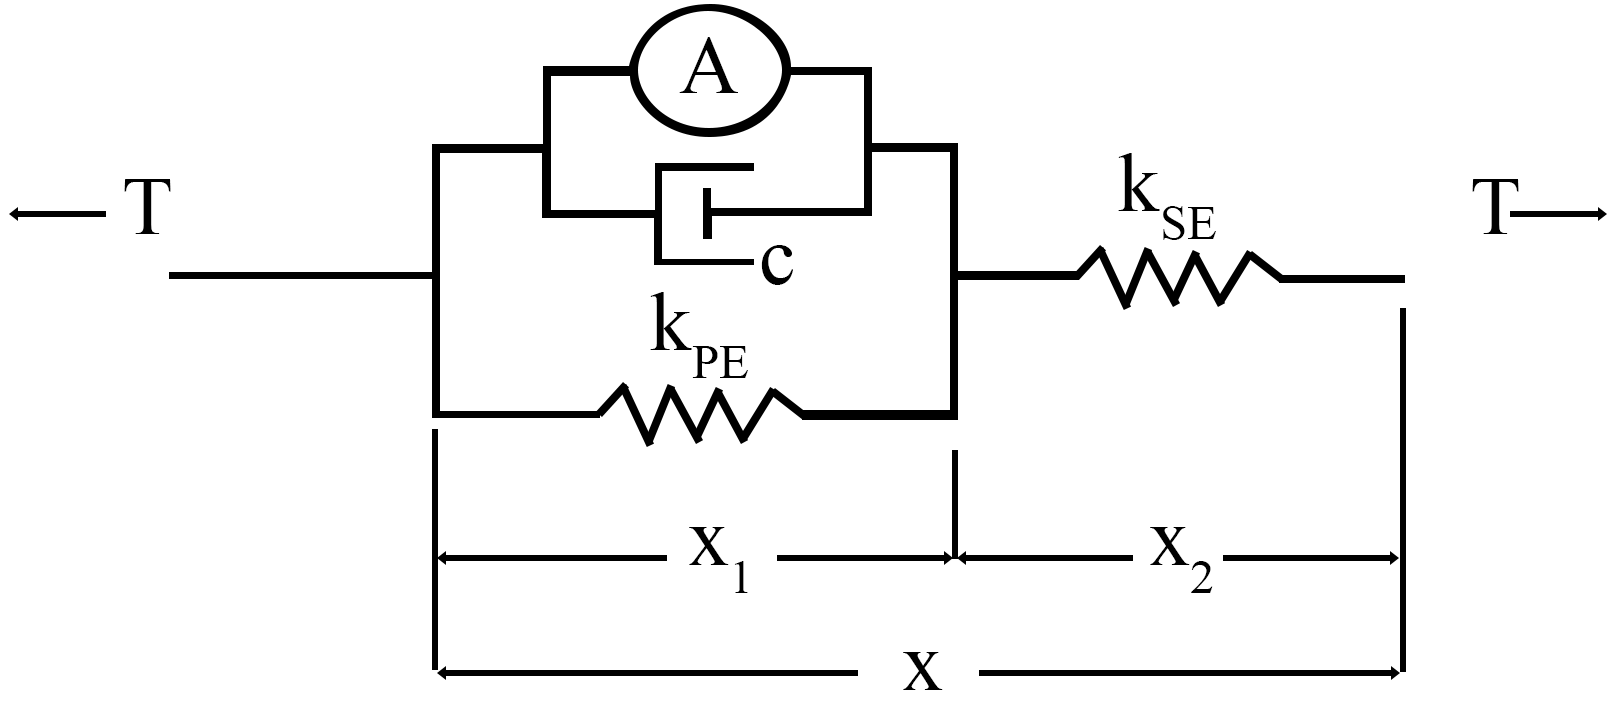
\includegraphics[width=.8\textwidth]{Figures/hill1.png}
		\caption{The Linear Hill Muscle Model}
		\label{fig:hill}
	\end{figure} \par
Where $T$ is the muscle tension, $k_{SE}$ is the serial element stiffness, $k_{PE}$ is the parallel element stiffness, $c$ is the muscle damping, $A$ is the active muscle unit, $L$ is the length of the muscle, $L_{rest}$ is the length of muscle at which tension is zero. This model demands explicit statements for these different variables, a data set that has not been found in the literature. By using muscle parameters examined by Johnson\cite{johnson_application_2011} and Eng\cite{eng_scaling_2008}, it is possible to develop these muscle parameters. Using the guidance of Zajac\cite{zajac_muscle_1989}, these muscle parameters were related to Hill parameters. Individual parameters are discussed individually as follows. \par

	\subsubsection{Serial Element Stiffness}
		The series elastic element (Kse) represents the tendon stiffness of the muscle. By using the tendon slack length (TSL) for each muscle\cite{johnson_application_2011}, the serial element stiffness was calculated from a generic stress-strain curve\cite{zajac_muscle_1989}, shown in Figure \ref{fig:stress-strain}. Normalized tendon stress equals normalized tendon force under the assumption that the optimal tendon stress is 32MPa.
			
			\begin{figure}[!htbp]
			    \begin{minipage}{0.5\textwidth}
			        \centering
			        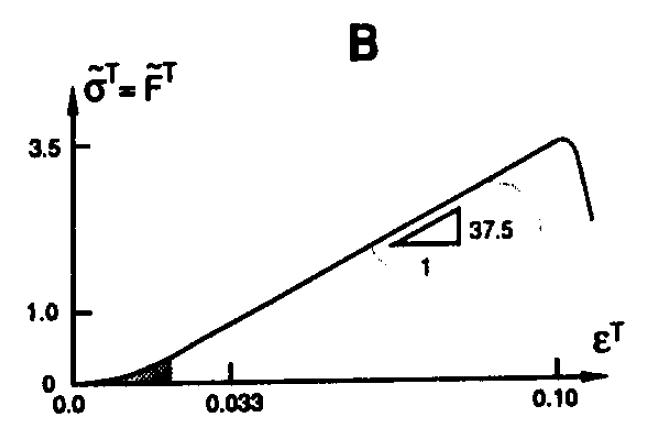
\includegraphics[width=\textwidth]{Figures/zajac1.PNG}
			        \caption{Zajac's normalized stress-strain curve.}
			        \label{fig:stress-strain}
			    \end{minipage}\hfill
			    \begin{minipage}{0.5\textwidth}
			        \centering
			        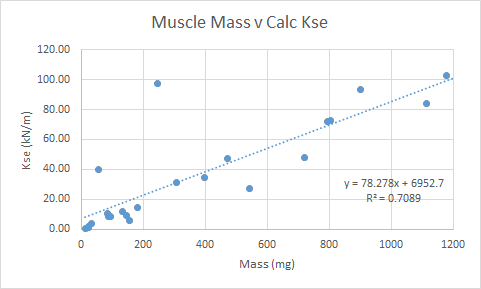
\includegraphics[width=\textwidth]{Figures/zajac3.png}
			        \caption{Zajac2}
			        \label{fig:img2}
			    \end{minipage}
			\end{figure}
			
		 Under the assumption that within the range of [1, 3.5]$F_{max}$, nominal tendon strain is [3.3,10]\%:
			\begin{align*}
				\epsilon^{T} &= \frac{\Delta L^{T}}{L_{s}^{T}}
				= \frac{L^{T}-L_{s}^{T}}{L_{s}^{T}}
				= \frac{L^{T}}{L_{s}^{T}} - 1 \\
				K_{se} &= \frac{\Delta F}{\Delta L}
				= \frac{\Delta F}{(\Delta \epsilon+1)L_{s}^{T}}
				= \frac{3.5 F_{o}^{M} - F_{o}^{M}}{1.1 L_{s}^{T} - 1.033 L_{s}^{T}}
				= 37.5 \frac{F_{o}^{M}}{L_{s}^{T}}
			\end{align*}
		where $\epsilon^{T}$ is the normalized tendon strain, $L^{T}$ is the tendon length, and $L_{s}^{T}$ is the TSL. While this calculation is convenient for muscles with defined TSL, many muscles lack a reliable TSL measurement. For these muscles, a trendline was established between muscle mass and $k_{SE}$.
	\subsubsection{Parallel Element Stiffness}
		The parallel elastic element can be calculated if we assume that the series and parallel elastic elements absorb all tension when the muscle is at a set length. By this assumption, we can treat the muscle as a simple two-spring system under load. Assuming the muscle exerts 70\% of their maximum force when fully contracted and knowing the values of $K_{se}$, we can find $K_{pe}$.
			\begin{align*}
				F &= K_{eq} x \\
				\Delta F &= K_{eq} \Delta L \\
				(F_{max} - .7 F_{max}) &= K_{eq} (L_{max}-L_{min}) \\
				.3 F_{max} &= \frac{K_{se}K_{pe}}{K_{se}+K_{pe}} (L_{max}-L_{min}) \\
				K_{pe} &= \frac{.3 F_{max} K_{se}}{K_{se} (L_{max}-L_{min})- .3 F_{max}}
			\end{align*}
		where $F_{max}$ is the maximum muscle force\cite{johnson_application_2011}, $K_{se}$ is the series element stiffness, and the length limits determined by computing the muscle length profiles.
	\subsubsection{Damping}
		\begin{align*}
			c &= \frac{F_{max}}{v_{f}^{M}*\big(\frac{L_{f}}{L_{m}}\big)} \\
			c &= \frac{F_{max}}{v_{max}} \\
		\end{align*}
	\subsubsection{Muscle Tension Curves}
		\paragraph{Length-Tension Curve}
			The length-tension (LT) curve of muscle is used to map the length of the muscle to to its force-generating capabilities. A general form of a muscle's LT curve\cite{zajac_muscle_1989} is shown in Fig. \ref{fig:lwidth3}. At an optimal resting length, a muscle is capable of producing an optimal isometric force. Above or below this optimal length, the muscle's ability to produce force is diminished. As the muscle is pulled to a supraoptimal length, passive forces within the muscle begin to accumulate, enhancing the muscle's ability to generate tension simply due to its structure. Animatlab presents a simplified version of the LT curve, shown in Fig. \ref{fig:lwidth3}. The muscle width is a property that Animatlab uses to define its simplified length-tension curve.  \par
			\begin{figure}
				\centering
				\begin{minipage}{0.53\textwidth}
					\centering
					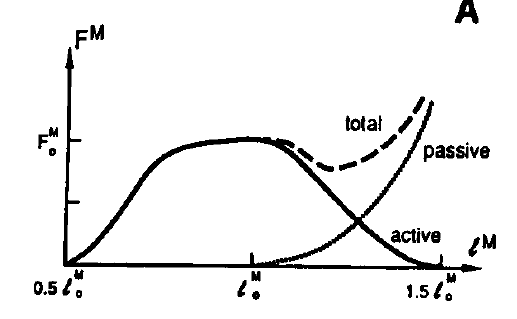
\includegraphics[width=.7\textwidth]{Figures/lwidth3.PNG}
					\caption{Nominal length-tension curve for muscle}
					\label{fig:lwidth3}
				\end{minipage}\hfill
				\begin{minipage}{0.47\textwidth}
					\centering
					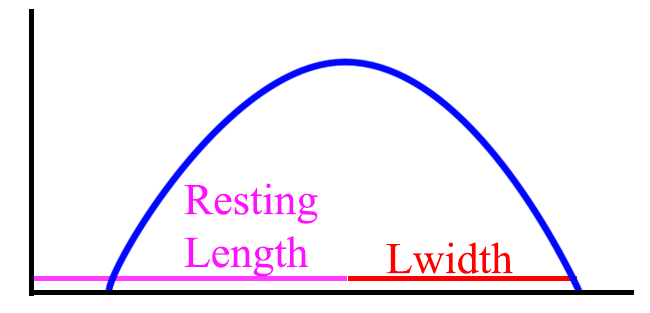
\includegraphics[width=\textwidth]{Figures/lwidth7.png}
					\caption{Simplified LT curve in Animatlab}
				\end{minipage}
			\end{figure}
			All muscle activity occurs within the ascending limb of the LT curve, meaning the muscle only becomes stronger as it is elongated to its maximum length. For a given walking profile (which determines the muscle length profile), every muscle is capable of generating 70\% of its maximum tension at its minimum length and 100\% of its maximum tension at its maximum length. Based on these assumptions and Animatlab's LT formula, $L_{width}$ can be calculated for each muscle:
				\begin{align*}
					T(L) &= \big(1-\frac{(L-L_{rest})^2}{L_{width}^2}\big)*100 \\
					.3 &= \frac{(L_{min}-L_{max})^2}{L_{width}^2} \\
					L_{width} &= \frac{|L_{min}-L_{max}|}{\sqrt{.3}} \\
		 			L_{width} &= \frac{|L_{min}-L_{max}|}{\sqrt{.3}}
				\end{align*}
		\FloatBarrier
		\paragraph{Stimulus-Tension Curve}
			The stimulus tension (ST) curve relates the membrane voltage of the motor neuron to the muscle tension. Other parameters from the ST equation include the maximum force amplitude, the steepness of the sigmoid, the x offset (in V), and the y-offset (in N).
			\begin{figure}
				\centering
				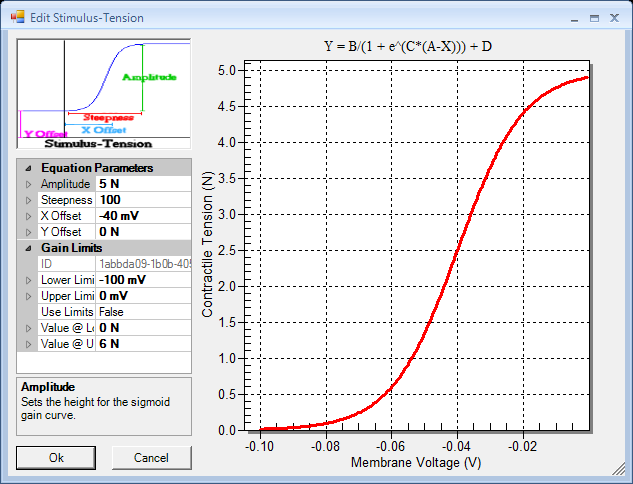
\includegraphics[width=.8\textwidth]{Figures/st2.PNG}
				\caption{The Animatlab stimulus-tension curve}
				\label{fig:STanim}
			\end{figure}
			We are able to find the parameters for the ST curve under two assumptions. First, under the operating voltage of [-.01,-.1] mV, the contractile tension grows from 0\% to 99\% of the maximum tension. Second, that the ST curve should be centered at -50 mV. Based on these assumptions, the steepness and y-offset of the curve can be determined:
			\begin{align*}
				T(V) &= \frac{Amplitude}{1+e^{(x_{offset}-V)*steepness}}+y_{offset} \\
					 &= \frac{F_{max}}{1+e^{(x_{offset}-V)S}}+y_{offset} \\
				T(-.01) = .99F_{max} &= \frac{F_{max}}{1+e^{-.04S}}+y_{offset} \\
				T(-.1) = 0 &= \frac{F_{max}}{1+e^{.05S}}+y_{offset} \\
				.99F_{max} &= \frac{F_{max}}{1+e^{-.04S}} - \frac{F_{max}}{1+e^{.05S}} \\
				.99 &= \frac{1}{1+e^{-.04S}} - \frac{1}{1+e^{.05S}} \\
				S &= 121.465 \\
				\\
				.99F_{max} &= \frac{F_{max}}{1+e^{-.04S}}+y_{offset} \\
				.99F_{max} &= \frac{F_{max}}{1+e^{-4.858}}+y_{offset} \\
				y_{offset} &= F_{max}\bigg(.99-\frac{1}{1+e^{-4.858}}\bigg) \\
				y_{offset} &= -.002294 F_{max}
			\end{align*}
	\subsubsection{Muscle Moment Arms}
		As a natural progression of analyzing the biomechanics of the model, the development of moment arm profiles during gait was developed. A moment arm calculation process developed from fundamental principles is a useful tool for analyzing the force generating capabilities of specific muscles in the model. This work led to a publication in the Journal of Biomimetics\cite{young_analyzing_2019}. \par
		Muscle moment arms are developed by projecting muscle paths onto a plane on interest and then measuring the shortest distance from the joint center to the free muscle segment. In the case of 2D walking, the plane of interest is the sagittal plane. Since muscles often contain multiple via points and those via points are often stationary relative to one another, the moment arm was calculated based on the segment of muscle that actively undergoes contraction during walking.
			\begin{figure}
				\centering
				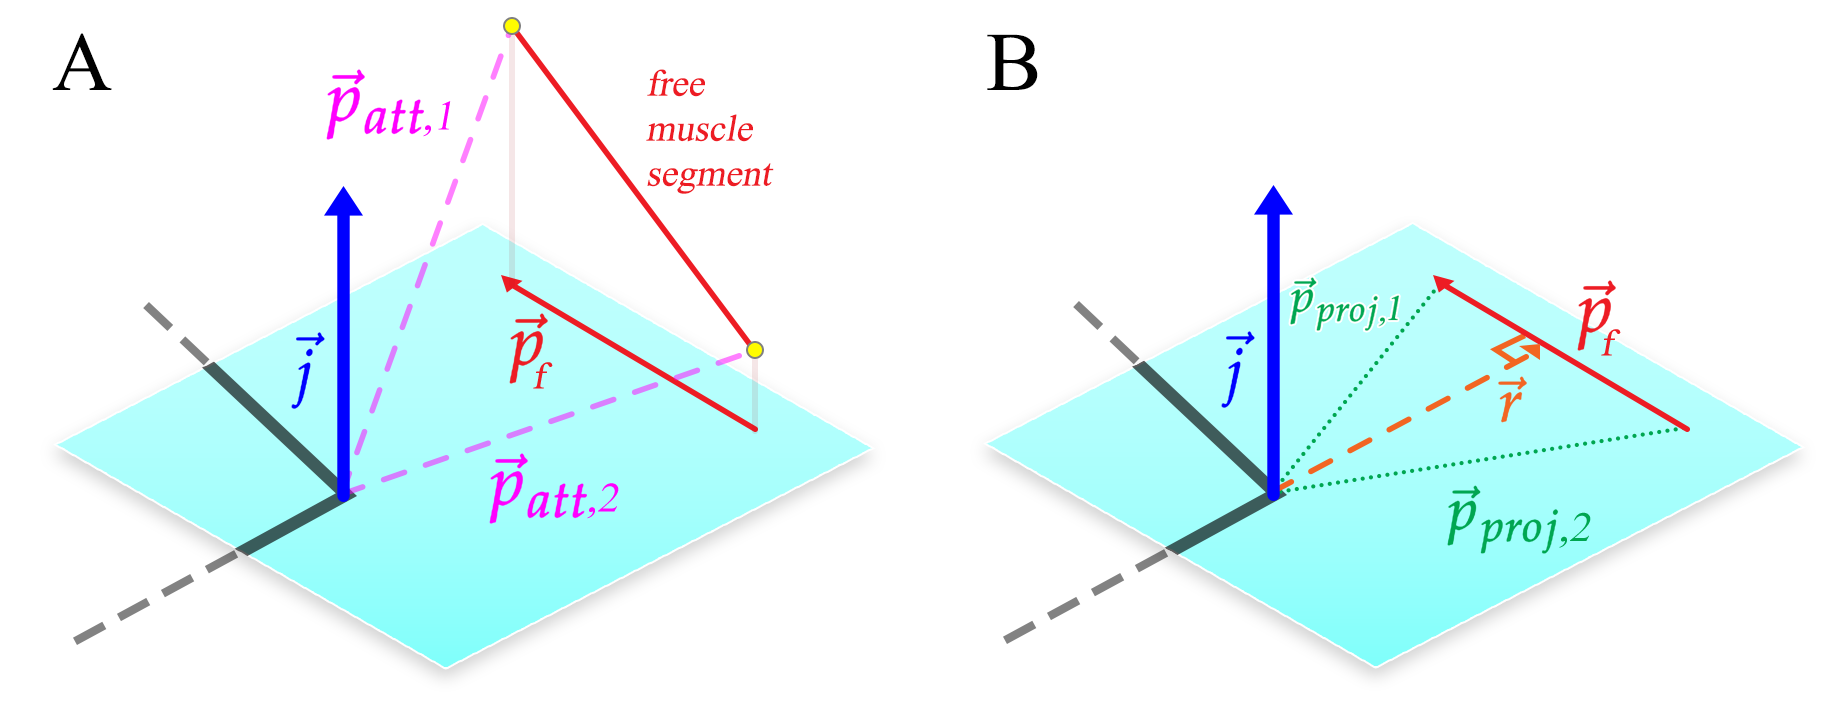
\includegraphics[width=.8\textwidth]{Figures/momarm1.png}
				\caption{The moment arm calculation example}
				\label{fig:momentarmexample}
			\end{figure}
\subsection{Aim 2 - Calculate motorneuron activation profiles for complete hindlimb actuation}
		The simplest method of developing motorneuron signals is to first calculate joint torque about each joint and then decompose the total torque profile into individual muscle forces. This decomposition process has an infinite solution set, as individual muscle contributions can be combined in infinite permutations to generate the torque profile. First, an accurate total torque profile was established based on data from project collaborators. Next, the biomechanics of the system were considered to determine the impact of passive and active torque on the system. Finally, the complete torque profile was decomposed into individual muscle forces through a linear optimization technique. \par 
		The overall torque profile was calculated for both the stance and swing phase of walking. Stance phase mean joint torque was calculated for rat hindlimb joints during graded walking\cite{andrada_biomechanics_2013}. A Simulink model of the hind limb was was developed to determine joint torque during swing phase. \par
		To determine torque generating muscle contributions, the passive torque due to body weight must be removed from the overall signal. Using ground reaction forces, it is possible to treat the leg like a multi-segmented arm with a force at the end effector.  Joint torques can be calculated by constructing a spatial manipulator Jacobian\cite{murray_mathematical_1994}, which combines the joint axes and positions. The composition of the spatial manipulator Jacobian is a 6$\times$n matrix of the form:
			\begin{align*}
				\textbf{J}^{s}_{st} =
				\begin{bmatrix}
					-\overrightarrow{\omega_{n}} \times \overrightarrow{q_n} \\
					\overrightarrow{\omega_{n}}
				\end{bmatrix}.
			\end{align*}
			where $\omega$ represents the joint axis and $q_{n}$ represents a joint's global coordinates.
		Load torques are calculated using ground reaction force data\cite{muir_ground_1999} from the literature. With the spatial manipulator Jacobian and the ground reaction forces, the sagittal plane load torque in all three joints can be calculated using,
			\begin{align*}
				\overrightarrow{\tau} &= (\textbf{J}^{s}_{st})^{T}\overrightarrow{F_{s}}.
			\end{align*}
		Active joint torque is the summation of individual muscle torques about each joint. With a method for calculating muscle moment arms in place, the only thing left is to calculate the muscle forces to generate the total torque profile. However, this is an infinite solution space making the outright distribution of muscle forces difficult. To address this problem a linear optimization has been applied. \par
		Linear optimization is appropriate for this problem since it involves the summation of torques. The only difficulty remaining is determining the ideal cost function. The linear optimization process follows the form
			\begin{align*}
				min\;f^{T} x\;such\;that 
				\begin{cases} 
				 	\mathbf{A_{eq}} \cdot \overrightarrow{x} = \overrightarrow{b_{eq}} \\
					\overrightarrow{lb} \leq \overrightarrow{x} \leq \overrightarrow{ub} 
				\end{cases}
			\end{align*}
		For this application, the muscle forces are represented by the vector $\overrightarrow{x}$, the muscle moment arms are compiled in $\mathbf{A_{eq}}$, and the torques are stored in $\overrightarrow{b_{eq}}$. 
			\begin{align*}
				{\setlength\extrarowheight{8pt}\begin{bmatrix}
					\sum_{i=1}^{38} p_{1,i} F_{i} \\
					\sum_{i=1}^{38} p_{2,i} F_{i} \\
					\sum_{i=1}^{38} p_{3,i} F_{i}
				\end{bmatrix}} =
				\begin{bmatrix}
					\tau_{1} \\
					\tau_{2} \\
					\tau_{3}
				\end{bmatrix}
			\end{align*}
		Where we're seeking to minimize some function, for example the sum of the muscle forces:
			\begin{align*}
				min\;\sum_{i=1}^{38} F_{i} 
			\end{align*}
		The results of this minimization are promising and demonstrate a rudimentary capability of distributing muscle forces to accommodate the torque profile. However, this method results in force profiles with a number of biologically unrealistic results. First, oftentimes muscle becomes saturated at the maximum for for extended periods of time, seeming to "plateau" while moving the joint. Second, complementary muscles tend to switch on and off rapidly, rather than a smooth, gradual hand off of responsibility. Third, not all muscles are represented in the force profile. Although it's to be expected that not every single muscle is activated throughout walking, one would expect that all muscles would contribute \textit{something} to locomotion at some point. 
		
	\bibliography{ThesisProposalReferences} 
	\bibliographystyle{ieeetr}
		
\end{document}